\documentclass[conference]{IEEEtran}

% Generated from the canonical modular manuscript; do not edit directly.

% This file embeds all result macros, sections, appendices, and references.

\usepackage{amsmath,amssymb}
\usepackage{booktabs}
\usepackage{cite}
\usepackage{graphicx}
\usepackage{microtype}
\usepackage{tikz}
\usepackage{pgfplots}
\usepackage{url}

\usetikzlibrary{arrows.meta,positioning,fit,shapes.geometric}
\pgfplotsset{compat=1.18}

\newcommand{\DB}{\textsc{DiffusionBlocks}}
\newcommand{\Exact}{\textsc{Exact}}
\newcommand{\ExactGraph}{\textsc{ExactGraph}}
\newcommand{\ZG}{\textsc{ZeroGraph}}
\newcommand{\E}{\mathbb{E}}

% Embedded machine-generated result macros.

% Generated from artifacts/modal_l4_stopped_seed1; do not hand edit.
\newcommand{\LFourTokens}{1,000,192}
\newcommand{\LFourSteps}{3,907}
\newcommand{\LFourBaselineHBM}{14.71 GiB}
\newcommand{\LFourZeroGraphHBM}{6.11 GiB}
\newcommand{\LFourMemoryReduction}{2.41\(\times\)}
\newcommand{\LFourBaselineSeconds}{5539.30 s}
\newcommand{\LFourZeroGraphSeconds}{879.06 s}
\newcommand{\LFourSpeedup}{6.30\(\times\)}
\newcommand{\LFourBaselineCE}{3.6342}
\newcommand{\LFourZeroGraphCE}{10.4811}
\newcommand{\LFourBaselinePPL}{37.87}
\newcommand{\LFourZeroGraphPPL}{35633.95}
\newcommand{\LFourBaselineAccuracy}{34.89\%}
\newcommand{\LFourZeroGraphAccuracy}{5.74\%}
\newcommand{\LFourInitialMSE}{100.0182}
\newcommand{\LFourFinalMSE}{0.5638}
\newcommand{\LFourMSEReduction}{99.44\%}
\newcommand{\LFourBaselineGenerativeCE}{2.1558}
\newcommand{\LFourZeroGraphGenerativeCE}{7.5821}
\newcommand{\LFourGenerativeDelta}{+5.4263}
\newcommand{\LFourAllreduce}{72.58 TB}
\newcommand{\LFourBaselineGPUHours}{6.155}
\newcommand{\LFourZeroGraphGPUHours}{0.974}
\newcommand{\LFourBaselineGPUHoursIncludingIO}{6.610}
\newcommand{\LFourZeroGraphGPUHoursIncludingIO}{1.210}
\newcommand{\LFourZeroGraphCheckpointGB}{17.61 GB}
\newcommand{\LFourBaselineCheckpointGB}{9.29 GB}
\newcommand{\LFourCheckpointRatio}{1.90\(\times\)}
\newcommand{\LFourLocalGate}{pass}
\newcommand{\LFourDenoisingGate}{pass}
\newcommand{\LFourContextGate}{fail}
\newcommand{\LFourRetentionGate}{fail}
\newcommand{\LFourMemoryGate}{pass}
\newcommand{\LFourSpeedGate}{pass}
\newcommand{\LFourAllGates}{fail}

% Generated by generate_tinyllama_results.py; do not hand edit.
\newcommand{\TinyParams}{1.100B}
\newcommand{\TinyTokens}{2,097,152}
\newcommand{\TinyOrdinaryHBM}{12.32 GiB}
\newcommand{\TinyAnchoredHBM}{2.67 GiB}
\newcommand{\TinyMemoryReduction}{4.62$\times$}
\newcommand{\TinyOrdinarySeconds}{1936.41 s}
\newcommand{\TinyAnchoredSeconds}{395.20 s}
\newcommand{\TinyComputeSpeedup}{4.90$\times$}
\newcommand{\TinyBaseCE}{1.6813}
\newcommand{\TinyTeacherCE}{1.3256}
\newcommand{\TinyOrdinaryCE}{1.2791}
\newcommand{\TinyAnchoredCE}{1.3096}
\newcommand{\TinyConfirmCE}{1.3574}
\newcommand{\TinyContextDelta}{0.8279}
\newcommand{\TinyAnchoredTeacherGenCE}{0.8892}
\newcommand{\TinyTeacherGenCE}{0.5967}
\newcommand{\TinySpend}{\$3.39}
\newcommand{\TinyBoundaryMSEMax}{0.0026}
\newcommand{\TinyUtilizationRange}{70.1--85.5\%}
\newcommand{\TinyPowerRange}{59.4--68.1 W}
\newcommand{\TinyCachedHashMatch}{4/4}
\newcommand{\TinyInterBlockBytes}{0}

% Generated from VERIFIED-SUMMARY.json; do not edit manually.
\newcommand{\SixACE}{1.4643}
\newcommand{\SixAPPL}{4.324}
\newcommand{\SixAAccuracy}{64.78\%}
\newcommand{\SixAHBM}{5.18~GiB}
\newcommand{\SixASeconds}{3564.4~s}
\newcommand{\SixCCE}{1.3059}
\newcommand{\SixCPPL}{3.691}
\newcommand{\SixCAccuracy}{67.57\%}
\newcommand{\SixCHBM}{5.13~GiB}
\newcommand{\SixCSeconds}{536.7~s}
\newcommand{\SixDCE}{1.3173}
\newcommand{\SixDPPL}{3.733}
\newcommand{\SixDAccuracy}{67.26\%}
\newcommand{\SixDHBM}{5.13~GiB}
\newcommand{\SixDSeconds}{531.3~s}
\newcommand{\SixECE}{1.3173}
\newcommand{\SixEPPL}{3.733}
\newcommand{\SixEAccuracy}{67.26\%}
\newcommand{\SixEHBM}{7.18~GiB}
\newcommand{\SixESeconds}{578.9~s}
\newcommand{\SixFCE}{1.3366}
\newcommand{\SixFPPL}{3.806}
\newcommand{\SixFAccuracy}{66.61\%}
\newcommand{\SixFHBM}{4.75~GiB}
\newcommand{\SixFSeconds}{2184.6~s}
\newcommand{\SixBaseCE}{1.6813}
\newcommand{\SixTeacherCE}{1.3256}
\newcommand{\SixBCE}{1.5554}
\newcommand{\SixCDDelta}{-0.0114}
\newcommand{\SixADDelta}{-0.1470}
\newcommand{\SixDEDelta}{0.0000}
\newcommand{\SixDFDelta}{-0.0194}
\newcommand{\SixMemoryRatio}{1.011$\times$}
\newcommand{\SixCMemoryRatio}{1.011$\times$}
\newcommand{\SixSpeedRatio}{6.709$\times$}
\newcommand{\SixFirstUseSeconds}{868.3~s}
\newcommand{\SixFirstUseRatio}{4.105$\times$}
\newcommand{\SixCFirstUseSeconds}{873.8~s}
\newcommand{\SixCFirstUseRatio}{4.079$\times$}
\newcommand{\SixOnlineRatio}{1.090$\times$}
\newcommand{\SixOnlineMemoryRatio}{1.400$\times$}
\newcommand{\SixHierarchyRatio}{4.112$\times$}
\newcommand{\SixCacheGiB}{40.0~GiB}
\newcommand{\SixCacheSeconds}{337.0~s}
\newcommand{\SixReuseTwoSeconds}{699.8~s}
\newcommand{\SixReuseEightSeconds}{573.4~s}
\newcommand{\SixBreakEvenReuse}{8}
\newcommand{\SixACollectiveTiB}{18.44~TiB/rank}
\newcommand{\SixDContextDelta}{7.3563}
\newcommand{\SixDShiftTeacher}{0.006398}
\newcommand{\SixDShiftStudent}{0.017747}
\newcommand{\SixDShiftRatio}{2.77$\times$}
\newcommand{\SixConfirmationCE}{not run}
\newcommand{\SixConfirmationGate}{not run (primary gate failed)}
\newcommand{\SixSpend}{\$8.09}
\newcommand{\SixParity}{all four blocks}
\newcommand{\SixInterBlock}{zero}

% Generated; do not edit. Source: VERIFIED-SUMMARY.json
\newcommand{\CampaignSpend}{33.01}
\newcommand{\CampaignCacheGiB}{72.0}
\newcommand{\CampaignCacheSeconds}{618.3}
\newcommand{\CampaignZGCE}{1.2779}
\newcommand{\CampaignFSDPCE}{1.4377}
\newcommand{\CampaignZeroThreeCE}{1.4399}
\newcommand{\CampaignGlobalCE}{1.3093}
\newcommand{\CampaignZGFirstUse}{1169.5}
\newcommand{\CampaignZGReuse}{551.1}
\newcommand{\CampaignFSDPTime}{5034.3}
\newcommand{\CampaignZeroThreeTime}{3496.5}
\newcommand{\CampaignGlobalFirstUse}{5275.3}
\newcommand{\CampaignZGPeak}{7.45}
\newcommand{\CampaignFSDPPeak}{7.47}
\newcommand{\CampaignZeroThreePeak}{11.52}
\newcommand{\CampaignGlobalPeak}{10.71}
\newcommand{\CampaignKOne}{724.0}
\newcommand{\CampaignKTwo}{412.9}
\newcommand{\CampaignKFour}{256.6}
\newcommand{\CampaignKEight}{176.5}
\newcommand{\CampaignKSixteen}{137.8}
\newcommand{\CampaignOnlineSixteen}{116.4}
\newcommand{\CampaignBTwoCE}{1.2937}
\newcommand{\CampaignBFourCE}{1.2779}
\newcommand{\CampaignBEightCE}{1.2742}
\newcommand{\CampaignThreeBCE}{1.3002}
\newcommand{\CampaignThreeBBaseCE}{1.2309}
\newcommand{\CampaignThreeBTeacherCE}{1.3600}
\newcommand{\CampaignThreeBPeak}{13.59}
\newcommand{\CampaignThreeBWall}{777.1}
\newcommand{\CampaignThreeBCacheGiB}{10.0}
\newcommand{\CampaignThreeBContext}{0.509}
\newcommand{\CampaignDownstreamZG}{0.646}
\newcommand{\CampaignDownstreamFSDP}{0.628}
\newcommand{\CampaignRestartHash}{238f1f1d7e3e}

\title{ZeroGraph: Replacing the Global Backward Graph\\
with Materialized Supervision}

\author{\IEEEauthorblockN{Omar Ramadan}
\IEEEauthorblockA{Independent Researcher}}

\begin{document}
\maketitle

\begin{abstract}
End-to-end backpropagation turns model depth into a synchronous information
dependency: an upstream update cannot be computed until downstream credit
arrives.  \ZG{} changes this systems contract by partitioning residual depth
into independently optimized denoising jobs with disjoint parameter ownership,
no inter-block autograd edges, and zero strict-mode inter-block gradient
traffic.  Independence alone is insufficient, however, because useful
intermediate semantics must still compose.  A preregistered GPT-2 Large
experiment on four disjoint L4 GPUs reduced peak allocated HBM by
\LFourMemoryReduction{} and shortened the measured local critical path by
\LFourSpeedup{} relative to matched DDP, yet failed context-use and
generation-retention gates: every local loss improved while all measured
low-noise context effects were negative.  We therefore replace the missing
online dependency with cached, noise-conditioned teacher boundary targets.  In
a revision-pinned \TinyParams{} TinyLlama/UltraChat conversion, this
materialized-supervision regime used \TinyMemoryReduction{} less peak HBM and
had a \TinyComputeSpeedup{} shorter local critical path than matched DDP.
Assembled held-out cross entropy was \TinyAnchoredCE{}, versus
\TinyOrdinaryCE{} for DDP and \TinyTeacherCE{} for the teacher; a confirmation
seed passed every preregistered gate.  Cache construction and assembly are
excluded from the local timing and remain explicit in our accounting. A new
six-arm, 2.10M-token comparison against four-way FSDP2 isolates the mechanism:
cached $\sigma=0$ boundary regression passed every generation gate at CE
\SixCCE{}, whereas cached and online noise-conditioned variants were bitwise
identical but both collapsed in free-running generation despite CE \SixDCE{}.
The successful boundary-regression arm's cache-inclusive first use was
\SixCFirstUseRatio{} shorter than FSDP2 in this allocation, while peak HBM was
essentially equal. A subsequent nine-phase Qwen2.5 campaign adds an
objective-matched cached/online comparison, ZeRO-3, $B\in\{2,4,8\}$,
boundary-shift sweeps, exact failure/restart, three seeds, and a real 3.086B
replication. Cached target acquisition was faster after materialization, but
did not break even by $K=16$; the 3B assembled model passed every quality gate
at CE \CampaignThreeBCE{} with zero inter-block gradient bytes. Thus
materialized trajectories create independently schedulable depth-wise jobs,
while neither a universal end-to-end speedup nor a benefit from the tested
language diffusion objective is established.
\end{abstract}

\begin{IEEEkeywords}
blockwise learning, distributed training, local objectives, materialized
supervision, knowledge distillation, memory-efficient training
\end{IEEEkeywords}

\section{Introduction}

Large-model systems usually optimize the mechanics of a globally connected
backward pass. Activation checkpointing trades recomputation for activation
storage~\cite{chen2016}; ZeRO and FSDP shard parameters, gradients, and
optimizer state~\cite{zero,fsdp}; tensor and pipeline parallelism distribute
operators and depth~\cite{megatron,gpipe}. These methods change where state
lives and when computation executes, but upstream credit still depends on
information produced downstream.

For ordinary reverse-mode differentiation, partition $b$ receives a cotangent
$\lambda_b=\partial\mathcal L/\partial h_b$ from the suffix. The cotangent may
be stored, recomputed, communicated, or losslessly encoded, but it cannot be
discarded while preserving the ordinary gradient for every downstream
computation. \ExactGraph{}, our objective-preserving control, rematerializes
partitions but retains this dependency.

\ZG{} takes the other branch of the design space: it changes the learning
signal so each partition can optimize without a downstream gradient. The
DiffusionBlocks construction assigns residual partitions denoising objectives
over noise intervals~\cite{diffusionblocks}. The systems appeal is immediate:
one backward graph and optimizer per block, zero strict-mode inter-block
gradient traffic, and one independently schedulable job per partition. The
scientific obligation is harder: independently learned representations must
still compose.

Our experiments isolate that obligation. Unanchored GPT-2 Large blocks reduce
their local losses and denoise targets while failing to use causal context or
retain language behavior. Removing the global backward signal removes not only
synchronization but also information constraining intermediate semantics. The
positive experiment supplies that information ahead of optimization through
\emph{materialized boundary supervision}. A frozen teacher is run once over a
fixed stream; its boundary states are cached; and block workers subsequently
train without the teacher body or neighboring trainable blocks:
\begin{equation}
\begin{gathered}
\text{synchronous backward cotangents}\\[-2pt]
\Downarrow\ \text{move cross-depth information in time}\ \Downarrow\\[-2pt]
\text{materialized boundary targets}
\end{gathered}
\label{eq:thesis}
\end{equation}

This is conversion/distillation, not from-scratch independent pretraining.
Teacher boundary matching itself is not claimed as novel. The systems
contribution is to make the materialized trajectory the cross-depth
information interface, changing \emph{when and where} global information is
delivered.

Our contributions are:
\begin{enumerate}
  \item We state the boundary between objective-preserving rematerialization
  and depth-independent optimization: exact upstream credit requires downstream
  information, while independent jobs require a replacement signal.
  \item We implement \ZG{} as a PyTorch partition/compiler runtime with
  explicit ownership, independent local jobs, resumable authenticated
  artifacts, and zero strict-mode inter-block autograd edges.
  \item We report a preregistered negative GPT-2 Large experiment showing that
  unanchored denoising can optimize locally while intermediate semantics drift.
  \item We isolate that signal in a six-arm TinyLlama comparison against
  four-way FSDP2: cached $\sigma=0$ boundary regression preserves coherent
  language, while adding the tested noise objective breaks free-running
  generation despite strong teacher-forced CE.
  \item We demonstrate bitwise equivalence of cached and online supervision,
  composition with inner FSDP2, explicit cache break-even accounting, a
  4.027B systems fixture, and a guarded 1.007B \ExactGraph{} certificate.
\end{enumerate}

\begin{figure*}[t]
\centering
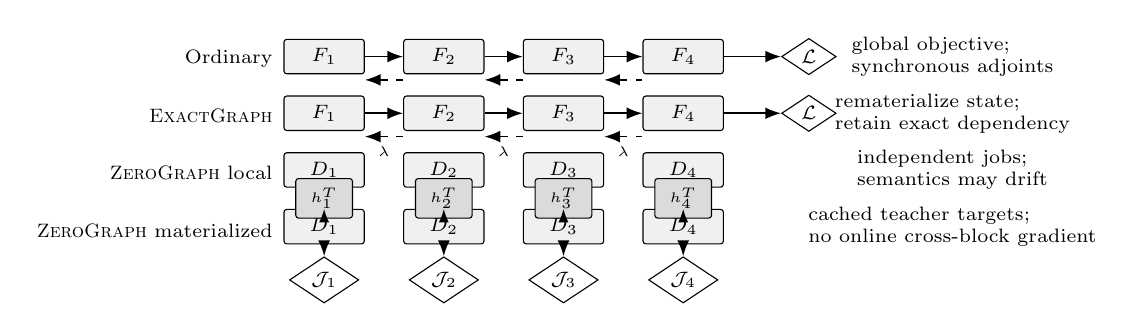
\begin{tikzpicture}[
 x=1.52cm,y=.72cm,
 block/.style={draw,rounded corners=1pt,minimum width=1.02cm,minimum height=.43cm,fill=black!6,font=\scriptsize},
 teach/.style={draw,rounded corners=1pt,minimum width=.72cm,minimum height=.34cm,fill=black!14,font=\tiny},
 loss/.style={draw,diamond,aspect=1.5,inner sep=1.4pt,font=\scriptsize},
 arr/.style={-{Latex[length=2mm]},semithick},
 grad/.style={{Latex[length=2mm]}-,dashed,semithick},
 sup/.style={-{Latex[length=1.7mm]},dotted,semithick},
 note/.style={font=\scriptsize,align=left}]
\node[note,anchor=e] at (-.35,3) {Ordinary};
\foreach \i/\k in {0/1,1/2,2/3,3/4} {\node[block] (o\i) at (\i,3) {$F_{\k}$};}
\node[loss] (ol) at (4.05,3) {$\mathcal L$};
\foreach \i/\j in {0/1,1/2,2/3} {\draw[arr] (o\i)--(o\j); \draw[grad] ([yshift=-2pt]o\i.south east)--([yshift=-2pt]o\j.south west);}
\draw[arr] (o3)--(ol);
\node[note] at (5.25,3) {global objective;\\synchronous adjoints};

\node[note,anchor=e] at (-.35,2) {\ExactGraph};
\foreach \i/\k in {0/1,1/2,2/3,3/4} {\node[block] (e\i) at (\i,2) {$F_{\k}$};}
\node[loss] (el) at (4.05,2) {$\mathcal L$};
\foreach \i/\j in {0/1,1/2,2/3} {\draw[arr] (e\i)--(e\j); \draw[grad] ([yshift=-2pt]e\i.south east)--node[below,font=\tiny] {$\lambda$}([yshift=-2pt]e\j.south west);}
\draw[arr] (e3)--(el);
\node[note] at (5.25,2) {rematerialize state;\\retain exact dependency};

\node[note,anchor=e] at (-.35,1) {\ZG{} local};
\foreach \i/\k in {0/1,1/2,2/3,3/4} {\node[block] (z\i) at (\i,1) {$D_{\k}$}; \node[loss,below=1.5mm of z\i] (zl\i) {$\mathcal L_{\k}$}; \draw[arr] (z\i)--(zl\i);}
\node[note] at (5.25,1) {independent jobs;\\semantics may drift};

\node[note,anchor=e] at (-.35,0) {\ZG{} materialized};
\foreach \i/\k in {0/1,1/2,2/3,3/4} {\node[block] (m\i) at (\i,0) {$D_{\k}$}; \node[teach] (t\i) at (\i,.50) {$h^T_{\k}$}; \node[loss,below=1.5mm of m\i] (ml\i) {$\mathcal J_{\k}$}; \draw[sup] (t\i)--(m\i); \draw[arr] (m\i)--(ml\i);}
\node[note] at (5.25,0) {cached teacher targets;\\no online cross-block gradient};
\end{tikzpicture}
\caption{Four execution semantics. Ordinary training and \ExactGraph{} retain
the reverse dependency required by the global objective. Unanchored \ZG{}
removes it but can lose compatible semantics. Materialized \ZG{} supplies a
cached reference trajectory while keeping block optimization independent.}
\label{fig:modes}
\end{figure*}

\section{From Backward Dependencies to Materialized Supervision}

Let a residual model be partitioned into $B$ contiguous maps
\begin{equation}
h_b=F_b(h_{b-1};\theta_b),\qquad b=1,\ldots,B,
\label{eq:chain}
\end{equation}
with ordinary loss $\mathcal L(h_B,y)$.

\subsection{The Objective-Preserving Boundary}

Reverse-mode differentiation applies
\begin{align}
g_b &= \left(\frac{\partial F_b}{\partial\theta_b}\right)^{\!T}\lambda_b,
&
\lambda_{b-1} &= \left(\frac{\partial F_b}{\partial h_{b-1}}\right)^{\!T}\lambda_b.
\label{eq:vjp}
\end{align}
Rematerialization can limit live state to a boundary and the partition being
recomputed, but it does not remove $\lambda_b$ as an information dependency.

\textit{Proposition 1 (reverse-dependency boundary).} Consider two
nonconstant differentiable partitions followed by an arbitrary differentiable
scalar loss. No algorithm updating the first partition from only its locally
visible forward information, while receiving neither a downstream adjoint nor
information sufficient to reconstruct it, can equal the ordinary gradient for
every suffix and loss.

\textit{Proof.} Hold the input, first partition, and all locally visible values
fixed. Choose two downstream compositions producing distinct cotangents at the
same boundary; opposite linear terminal losses after an identity suffix
suffice. A local algorithm must emit the same update because its observations
are identical, while the chain rule in (\ref{eq:vjp}) changes the gradient
whenever the local Jacobian has a component in the differing-adjoint direction.
At least one ordinary gradient cannot be reproduced. $\square$

The proposition marks a systems boundary rather than a new chain-rule result.
Exact execution may store, recompute, compress, or reconstruct the cotangent;
independent depth-wise optimization needs another learning signal.

\subsection{Unanchored Local Denoising}

For target representation $y$ and context $x$, sample
$z_\sigma=y+\sigma\epsilon$, where $\epsilon\sim\mathcal N(0,I)$. Following
score-based denoising~\cite{song,karras}, split the noise support into intervals
$I_b=[\sigma_b,\sigma_{b-1}]$. Block $b$ minimizes
\begin{equation}
\mathcal L_b(\theta_b)=\E\!\left[w(\sigma)
\ell(D_b(x,z_\sigma,\sigma;\theta_b),y)\right],\quad \sigma\sim p_b,
\label{eq:local}
\end{equation}
where $p_b$ is the base distribution restricted to $I_b$. With frozen or
block-private interfaces, $\mathcal L_b$ contains only $\theta_b$:
\begin{equation}
\frac{\partial\mathcal L_b}{\partial\theta_c}=0\;(c\ne b),\qquad
\nabla_\theta^2\sum_b\mathcal L_b\ \text{is block diagonal}.
\label{eq:independence}
\end{equation}
This gives zero inter-block gradient traffic. It does not require independently
learned boundary representations to remain mutually compatible.

\subsection{Materialized Boundary Supervision}

Let a frozen teacher define $h_0^T,\ldots,h_B^T$ on a fixed stream. Boundary
states are generated before local optimization and stored as targets. Worker
$b$ then minimizes
\begin{align}
z_{b,\sigma}^T &= h_b^T+\sigma\epsilon,\\
\mathcal J_b(\theta_b) &= \E\!\left[w(\sigma)\ell\!\left(
D_b(h_{b-1}^T,z_{b,\sigma}^T,\sigma;\theta_b),h_b^T\right)\right]
+R_b(\theta_b),
\label{eq:materialized}
\end{align}
where $R_b$ contains declared local regularizers or task terms. The TinyLlama
recipe includes a clean initialization anchor and final-block assistant cross
entropy. Once the cache exists, a worker needs neither the teacher body nor a
neighboring trainable block.

This regime moves global information; it does not erase it. It also introduces
a distribution shift: training conditions on $h_{b-1}^T$, whereas assembled
inference receives a learned predecessor state. We therefore measure assembled
boundary MSE and context ablations. Robustness to deliberately perturbed or
mixed teacher/assembled boundaries remains an open ablation.

\begin{table}[t]
\caption{Placement of cross-depth information.}
\label{tab:dependency}
\centering\footnotesize
\begin{tabular}{@{}llll@{}}
\toprule
Regime & Objective & Online signal & Local jobs \\
\midrule
Ordinary & global & $\lambda_b$ & no \\
\ExactGraph{} & global & exact $\lambda_b$ & no \\
\ZG{} unanchored & local & none & yes \\
\ZG{} materialized & teacher-local & cached $h_b^T$ & yes \\
\bottomrule
\end{tabular}
\end{table}

\section{Compiler, Runtime, and Cost Model}

The compiler captures an executable PyTorch model with
\texttt{torch.export}~\cite{pytorch}, identifies guarded residual separators,
assigns parameters, buffers, and aliases to explicit owners, and emits one
loadable artifact per block. Shape-changing heads and shared interfaces remain
explicit. Strict independence requires shared trainable interfaces to be
frozen or block-private; synchronization is possible but invalidates the
zero-inter-block-communication contract.

Teacher boundaries are bound to model and dataset revisions, sample order,
shapes, and content digests. Workers consume cached targets without loading the
teacher during timed updates. Checkpoints bind block identity, program digest,
optimizer, step, and RNG state. Training, assembly, quality evaluation, and
evidence verification are separate operations, preventing local loss from
standing in for assembled quality.

For block $b$ with $N_b$ parameters, effective state cost $s_{\rm state}$,
inner sharding degree $D_b$, and activation footprint $A_b$, active memory is
approximately
\begin{equation}
M_b\approx \frac{s_{\rm state}N_b}{D_b}+A_b+M_{\rm shared}+M_{\rm runtime}.
\label{eq:memory}
\end{equation}
FSDP/ZeRO, tensor/context parallelism, and activation checkpointing remain
applicable inside an oversized block. With disjoint hardware, local critical
time approaches $\max_bT_b$ rather than $\sum_bT_b$; aggregate work is not
thereby reduced.

Teacher materialization is not free. Let $T_{\rm cache}$ be cache generation,
$T_{\rm asm}$ assembly/evaluation, and $K$ the number of runs reusing a cache:
\begin{align}
T_{\rm ZG,total} &= T_{\rm cache}+\max_bT_b+T_{\rm asm},\\
\bar T_{\rm ZG}(K) &= \frac{T_{\rm cache}}{K}+\max_bT_b+T_{\rm asm}.
\label{eq:amortized}
\end{align}
If $T_{\rm local}=\max_bT_b+T_{\rm asm}<T_{\rm base}$, reuse breaks even only
when
\begin{equation}
K>\frac{T_{\rm cache}}{T_{\rm base}-T_{\rm local}}.
\label{eq:breakeven}
\end{equation}
The experiments report local critical paths, cache size, and accelerator-hours
separately; they do not establish favorable first-use end-to-end economics
against FSDP or ZeRO-3.

\section{Experimental Method}

\subsection{Unanchored GPT-2 Large Diagnostic}

The preregistered study uses revision-pinned GPT-2 Large (774,030,080
parameters) and a SHA-256-pinned ten-million-token GPT-2 encoding of
FineWeb-Edu. Each arm consumes 1,000,192 unique tokens at sequence length 64.
The control is four-rank DDP with activation checkpointing. The treatment maps
four nine-layer blocks to four disjoint L4 GPUs. Both arms execute the same
steps, unique tokens, and aggregate residual-layer--token traversals; duplicated
local vocabulary-interface work remains in the accounting.

The reported evidence is one completed matched seed (20260911). A planned
second seed and $B=2$ ablation were stopped for budget and excluded. Each local
block ran 3,907 AdamW steps at $5\times10^{-5}$ with BF16 compute. The objective
used equi-probability noise intervals, 5\% overlap, a weak $10^{-5}$
initialization anchor, and no teacher or context-margin term. Quality uses the
same 8,192 held-out tokens, fixed corruptions, contexts, and frozen source
scorer. Thresholds were locked before the completed arms.

\subsection{TinyLlama Materialized-Supervision Conversion}

The follow-up uses revision-pinned TinyLlama base (1,100,048,384 parameters),
TinyLlama Chat as frozen teacher, and UltraChat 200k. We deterministically
select 8,192 first-turn exchanges for training and 512 disjoint validation
examples at sequence length 256. The 22 decoder layers are partitioned
$[0,6),[6,12),[12,17),[17,22)$ across four L4s. The control is four-rank DDP.
Each treatment worker trains one base-initialized partition against cached
noise-conditioned teacher boundaries, a clean anchor, and final-block assistant
cross entropy. Teacher embedding, RMSNorm, and LM head are frozen.

The locked ladder uses 128-step pilots, a 2,048-step primary
(\TinyTokens{} tokens), and a 256-step confirmation seed. The unanchored pilot
cannot escalate when any learning, context, generation, or held-out gate fails.
The cached replay must reproduce the earlier online-reference checkpoint hashes
and assembled metrics. Five BF16 boundary tensors occupy 40~GiB of persistent
storage; cache creation is outside timed local updates.

\subsection{Six-Arm FSDP2 and Objective-Isolation Matrix}

We strengthen that comparison with six arms under the same pinned base,
teacher, dataset, 256-token shape, deterministic data stream, AdamW settings,
BF16 compute, and 2,097,152-token primary budget. Arm A replaces DDP with global
assistant-CE SFT using four-way FSDP2 and activation checkpointing. Arm B is the
unanchored four-block objective and is pilot-gated. Arm C trains the four
partitions against cached teacher boundaries only at $\sigma=0$. Arm D is
materialized \ZG{} with cached boundaries and log-uniform
$\sigma\in[0.005,0.10]$. Arm E recomputes D's targets from the teacher online.
Arm F changes D to $B=2$, with each independent block sharded over a disjoint
two-L4 FSDP2 group.

Thus A versus D is the strong conventional systems comparison; B tests whether
unanchored local denoising preserves language semantics; C versus D isolates
noise conditioning beyond hidden-state regression; D versus E isolates
materialization rather than objective; and D versus F tests composition with
state sharding. The initial 128-step gate and its post-pilot, append-only
256-step correction are disclosed in Appendix~\ref{app:six-arm}. Primaries
escalate only after the corrected learning and unchanged assembled-quality
gates pass. Evaluation includes held-out CE and accuracy, context ablation,
fixed-prompt generation, teacher-scored generations, and boundary mixtures
$\alpha h^T+(1-\alpha)h^{\rm assembled}$ for
$\alpha\in\{1,.75,.5,.25,0\}$. A second fixed seed confirms D. All timings
separate cache construction, local critical compute, evaluation, and
checkpoint I/O; FSDP2 tensor payload is labeled algorithmic rather than fabric
traffic.

\section{Results}

\subsection{Unanchored Blocks Optimize but Lose Semantics}

\begin{table*}[t]
\caption{Completed matched GPT-2 Large seed on four L4s. Compute excludes
checkpoint I/O; \ZG{} time is the slowest concurrent block.}
\label{tab:l4results}
\centering\footnotesize
\begin{tabular}{@{}lrrrrrr@{}}
\toprule
Arm & GPUs & $B$ & Peak HBM & Compute & Held-out CE & Accuracy \\
\midrule
DDP + checkpointing & 4 & 1 & \LFourBaselineHBM & \LFourBaselineSeconds & \LFourBaselineCE & \LFourBaselineAccuracy \\
\ZG{} unanchored & 4 & 4 & \LFourZeroGraphHBM & \LFourZeroGraphSeconds & \LFourZeroGraphCE & \LFourZeroGraphAccuracy \\
\bottomrule
\end{tabular}
\end{table*}

Table~\ref{tab:l4results} reports a \LFourMemoryReduction{} peak-HBM reduction
and \LFourSpeedup{} shorter local critical path. All four local loss windows
improved, and assembled denoising MSE fell from \LFourInitialMSE{} to
\LFourFinalMSE{}. Yet held-out CE rose from \LFourBaselineCE{} to
\LFourZeroGraphCE{}, and token accuracy fell from \LFourBaselineAccuracy{} to
\LFourZeroGraphAccuracy{}.

\begin{table}[t]
\caption{Predeclared GPT-2 Large gates.}
\label{tab:l4gates}
\centering\footnotesize
\begin{tabular}{@{}lll@{}}
\toprule
Gate & Threshold & Outcome \\
\midrule
Peak HBM & $\geq1.5\times$ reduction & \LFourMemoryGate{} \\
Critical compute & $\geq1.1\times$ shorter & \LFourSpeedGate{} \\
Local learning & all blocks improve & \LFourLocalGate{} \\
Assembled denoising & $\geq20\%$ MSE reduction & \LFourDenoisingGate{} \\
Low-$\sigma$ context & every block $>1\%$ & \LFourContextGate{} \\
Generation retention & $\Delta$CE $\leq2.0$ & \LFourRetentionGate{} \\
\bottomrule
\end{tabular}
\end{table}

Every low-noise context effect was negative ($-1.02\%$, $-1.03\%$, $-1.22\%$,
and $-2.20\%$): bypassing context slightly improved denoising. The source model
scored ordinary continuations at CE \LFourBaselineGenerativeCE{} and \ZG{}
continuations at \LFourZeroGraphGenerativeCE{}. The combined gate status is
\LFourAllGates{}. Thus the blocks learned the corrupted target representation
without learning a compositionally useful causal transformation.

Strict \ZG{} reported zero inter-block gradient bytes. The DDP ring-allreduce
payload estimate was \LFourAllreduce{}; this is algorithmic, not fabric-counter
traffic. Excluding checkpoint I/O, DDP consumed \LFourBaselineGPUHours{}
accelerator-hours and \ZG{} consumed \LFourZeroGraphGPUHours{}. Duplicated local
interfaces increased final checkpoint storage from \LFourBaselineCheckpointGB{}
to \LFourZeroGraphCheckpointGB{}. Active HBM reduction is not storage reduction.

\subsection{Materialized Supervision Restores Composition}

The unanchored TinyLlama pilot failed generation coherence and did not escalate.
Every anchored pilot block learned, and the assembled model passed all gates.

\begin{table}[t]
\caption{TinyLlama primary on four L4s. Critical compute excludes cache
construction, loading, and checkpoint I/O.}
\label{tab:tinyllama}
\centering\footnotesize
\resizebox{\columnwidth}{!}{%
\begin{tabular}{@{}lrrr@{}}
\toprule
Arm & Peak HBM & Critical compute & Held-out CE \\
\midrule
Frozen base & --- & --- & \TinyBaseCE{} \\
Frozen Chat teacher & --- & --- & \TinyTeacherCE{} \\
Ordinary DDP SFT & \TinyOrdinaryHBM{} & \TinyOrdinarySeconds{} & \TinyOrdinaryCE{} \\
Materialized \ZG{} & \TinyAnchoredHBM{} & \TinyAnchoredSeconds{} & \TinyAnchoredCE{} \\
\bottomrule
\end{tabular}}
\end{table}

Anchored CE was \TinyAnchoredCE{}, 0.0305 nat above ordinary SFT and 0.0160
below the frozen teacher. The context-ablation delta was \TinyContextDelta{}
nat, with four of four positive prompt deltas; teacher-scored generation CE was
\TinyAnchoredTeacherGenCE{} versus \TinyTeacherGenCE{} for teacher generations.
The 256-step confirmation seed passed every gate at CE \TinyConfirmCE{}.

The cached replay reproduced \TinyCachedHashMatch{} online checkpoint hashes
and all held-out metrics; maximum assembled teacher-boundary MSE was
\TinyBoundaryMSEMax{}. Peak HBM fell by \TinyMemoryReduction{}, and the local
critical path was \TinyComputeSpeedup{} shorter, with \TinyInterBlockBytes{}
inter-block gradient bytes. The complete campaign cost \TinySpend{} under its
locked budget. These measurements establish one conversion recipe on one
architecture, not a universal speed or quality law.

\subsection{Strong FSDP2 and Objective Controls}

The six-arm matrix sharpens that result. Table~\ref{tab:six-arm} reports the
locked primaries; B is shown separately because its failed pilot could not
escalate. Every primary consumed 2,097,152 tokens. C, cached boundary regression
at $\sigma=0$, achieved the best CE (\SixCCE{}) and passed every context and
generation gate. D improved teacher-forced CE to \SixDCE{} and had a large
positive context-ablation effect (\SixDContextDelta{} nats), yet its free-running
outputs collapsed: maximum token share was 0.664 and repeated-bigram fraction
was 0.675. Its primary gate therefore failed, and the locked stop rule barred
the confirmation seed. F failed the same coherence gate.

\begin{table}[t]
\caption{TinyLlama six-arm comparison on four L4s. Time is the local critical
compute path and excludes cache construction, evaluation, and checkpoint I/O.}
\label{tab:six-arm}
\centering\footnotesize
\resizebox{\columnwidth}{!}{%
\begin{tabular}{@{}llrrrl@{}}
\toprule
Arm & Learning signal & Peak HBM & Time & CE & Generation \\
\midrule
A & global CE, FSDP2 & \SixAHBM{} & \SixASeconds{} & \SixACE{} & pass \\
C & cached boundary, $\sigma=0$ & \SixCHBM{} & \SixCSeconds{} & \SixCCE{} & pass \\
D & cached boundary + noise & \SixDHBM{} & \SixDSeconds{} & \SixDCE{} & fail \\
E & online boundary + noise & \SixEHBM{} & \SixESeconds{} & \SixECE{} & fail \\
F & D, $B=2$, inner FSDP2 & \SixFHBM{} & \SixFSeconds{} & \SixFCE{} & fail \\
\bottomrule
\end{tabular}}
\end{table}

This isolates the scientific contribution more narrowly. C minus D held-out CE
was \SixCDDelta{} nat, and only C generated coherently; under this recipe,
diffusion noise did not improve composition beyond FitNets-style boundary
regression. The unanchored B pilot likewise failed coherence at CE \SixBCE{}.
Materialized boundary supervision itself remains the positive result, while the
tested language DiffusionBlocks objective is a negative result.

Against the strong FSDP2 control, C's local path was \SixCSeconds{} and its
cache-inclusive first use was \SixCFirstUseSeconds{}, \SixCFirstUseRatio{}
shorter than A's \SixASeconds{} compute path in this allocation. Peak HBM was
nearly equal (A/C: \SixCMemoryRatio{}), so this experiment does \emph{not}
establish a memory advantage over four-way FSDP2. A's algorithmic collective
payload estimate was \SixACollectiveTiB{}; strict C/D/E and inter-block F
traffic were \SixInterBlock{}. These are tensor-payload estimates, not measured
fabric counters, and the comparison is conversion/distillation versus ordinary
SFT rather than objective parity.

D and E produced \SixParity{} in bitwise-equal canonical parameter states and
identical CE, proving that caching changed information placement rather than
the executed objective. Caching reduced peak HBM by \SixOnlineMemoryRatio{} and
made E's local path \SixOnlineRatio{} longer, but the 40-GiB cache cost
\SixCacheSeconds{} to create. It amortized below online recomputation only at
$K=\SixBreakEvenReuse{}$ among $K\in\{1,2,4,8\}$. F demonstrates that
independent objectives compose mechanically with inner FSDP2, but its
\SixHierarchyRatio{} longer critical path shows that this two-GPU-per-block L4
configuration was inefficient. At the final block, fully assembled predecessor
states increased D's boundary MSE from \SixDShiftTeacher{} to
\SixDShiftStudent{} (\SixDShiftRatio{}), quantifying train--inference boundary
shift. The complete locked campaign cost \SixSpend{}.

\subsection{Evidence-First Strengthening Campaign}

We next held the clean teacher-boundary signal fixed and changed only where it
was produced. Recomputed online boundaries and the persistent BF16 cache agreed
bitwise on all 12 tested boundaries (maximum MSE zero). Across 16 paired short
trials, cached jobs averaged 99.13~s after materialization versus 116.39~s
online. The 72.0-GiB cache cost \CampaignCacheSeconds{}~s to create, however,
so cache-inclusive amortized times at $K=1,2,4,8,16$ were \CampaignKOne{},
\CampaignKTwo{}, \CampaignKFour{}, \CampaignKEight{}, and
\CampaignKSixteen{}~s/run. Online averaged \CampaignOnlineSixteen{}~s at
$K=16$; no measured break-even occurred. Materialization shortened recurring
target acquisition and changed the dependency graph, but did not establish an
end-to-end wall-time advantage in this reuse range.

\begin{table}[t]
\caption{Qwen2.5-1.5B accounting on four L4s. First use includes cache
construction where applicable; reuse does not. SFT and distillation objectives
are not treated as objective matched.}
\label{tab:campaign-systems}
\centering\scriptsize
\resizebox{\columnwidth}{!}{%
\begin{tabular}{@{}lrrrr@{}}
\toprule
Arm & First use & Reuse & Peak GiB & CE \\
\midrule
FSDP2 SFT & \CampaignFSDPTime & \CampaignFSDPTime & \CampaignFSDPPeak & \CampaignFSDPCE \\
ZeRO-3 SFT & \CampaignZeroThreeTime & \CampaignZeroThreeTime & \CampaignZeroThreePeak & \CampaignZeroThreeCE \\
Global boundary distill & \CampaignGlobalFirstUse & 4657.0 & \CampaignGlobalPeak & \CampaignGlobalCE \\
\ZG{} cached boundary & \CampaignZGFirstUse & \CampaignZGReuse & \CampaignZGPeak & \CampaignZGCE \\
\bottomrule
\end{tabular}}
\end{table}

The 16-pair cached/online block experiment is the strict objective-matched test;
Table~\ref{tab:campaign-systems} provides broader systems references. Five-task
zero-shot mean accuracy was \CampaignDownstreamZG{} for \ZG{} and
\CampaignDownstreamFSDP{} for FSDP2. The clean-boundary block-count sweep
passed all gates: held-out CE was \CampaignBTwoCE{}, \CampaignBFourCE{}, and
\CampaignBEightCE{} for $B=2,4,8$. Interpolating teacher and assembled
predecessor states increased late-boundary error as assembled-state weight grew,
directly connecting representation drift to boundary mismatch, although CE
remained stable in the measured range. This does not rescue the separate noisy
objective, whose free-running coherence failure replicated.

Qwen2.5-3B (3,085,938,688 parameters) then trained as four disjoint jobs for
2,048 updates each. Assembled CE was \CampaignThreeBCE{} versus
\CampaignThreeBBaseCE{} for the base and \CampaignThreeBTeacherCE{} for the
teacher; context delta was +\CampaignThreeBContext{} nat with four positive
prompt deltas. All gates passed, peak allocated HBM was \CampaignThreeBPeak{}
GiB, and inter-block gradient traffic was zero. This is real 3B
conversion/distillation, not from-scratch pretraining. Separately, one job was
killed by SIGTERM halfway and resumed with optimizer, RNG, and sample order;
its final state was bitwise identical to an uninterrupted deterministic control
(digest prefix \texttt{\CampaignRestartHash}). The other three jobs required no
retraining or rollback. The verified nine-phase campaign cost
\$\CampaignSpend{}.

\section{Related Work}

Checkpointing and dynamic rematerialization preserve the ordinary objective
while reducing activation retention~\cite{chen2016,dtr}; ZeRO, FSDP, Megatron,
and pipeline parallelism redistribute state or execution while retaining global
credit~\cite{zero,fsdp,megatron,gpipe}. \ExactGraph{} is our control in this
objective-preserving family.

Synthetic gradients and greedy layerwise learning reduce locking through local
or predicted signals~\cite{dni,greedy}. \ZG{} instead uses the DiffusionBlocks
noise-local objective~\cite{diffusionblocks}, grounded in score/SDE and EDM
denoising~\cite{song,karras}. BlockTrain independently studies local text
objectives and block-level transport~\cite{blocktrain}.

Knowledge distillation transfers behavior from teachers to students
~\cite{hinton2015}; FitNets and later Transformer distillation methods match
intermediate representations~\cite{fitnets,patientkd,tinybert}. We do not claim
teacher hidden-state targets as new. Our question is whether an authenticated,
reusable boundary trajectory can serve as the systems interface that removes
the teacher and neighboring trainable blocks from each local optimization loop.
The failure--repair sequence makes this distinction measurable: unanchored jobs
lose compatible semantics; materialized boundaries restore a reference
trajectory while preserving independent optimization.

\section{Limitations and Reproducibility}

The strongest positive result is teacher-anchored conversion, not from-scratch
pretraining. It covers one architecture, one 2.10M-token primary, and a short
confirmation seed. Teacher scoring and held-out CE do not replace broad
downstream or human evaluation. The executed recipe combines boundary targets,
clean anchoring, final-block assistant CE, and frozen interfaces; it establishes
sufficiency, not the marginal effect of each term.

Training uses teacher predecessor states while inference uses learned states.
The low assembled boundary MSE is encouraging but does not establish robustness
under accumulated boundary shift. The five cached tensors occupy 40~GiB, and
cache construction is excluded from the local critical-path comparison.
Equation~(\ref{eq:amortized}) was evaluated through $K=16$: cached execution
remained slower after amortizing construction, so no break-even is claimed.
The strengthening campaign adds ZeRO-3, three 1.5B seeds, and a real 3B
replication, but still covers only Qwen2.5-family models, short adaptation
budgets, one four-L4 provider topology, and automatic rather than human
language evaluation.

The six-arm result also narrows the algorithmic claim. Cached $\sigma=0$
boundary regression passed generation gates, while the executed noise-conditioned
D/E variants and hierarchical F variant did not. Their strong teacher-forced CE
and context-ablation scores therefore cannot be interpreted as usable language
quality. The preregistered stop rule barred D's confirmation after its primary
failure. C's positive result is hidden-state distillation used as a systems
interface, not evidence that diffusion is necessary, and its comparison with
ordinary SFT is not objective parity. F proves mechanical composition with
FSDP2 but was slower on the tested L4 allocation; no universal sharding law is
claimed.

The GPT-2 Large study has one completed seed; the planned replication and block
count ablation were not completed. Its negative outcome is diagnostic, not a
proof against all unanchored objectives. All numerical macros are generated
from retained evidence. The verifier checks 50 claims, cross-file invariants,
checkpoint identities, and complete source digests. The supplementary appendix
contains the ExactGraph control, 4.027B systems fixture, smaller studies,
expanded protocols, and traceability anchors.

\section{Conclusion}

Global backpropagation couples depth because upstream credit depends on
downstream information. Rematerialization can change storage and execution but
cannot make the ordinary objective depth-independent. \ZG{} changes the
contract. Unanchored GPT-2 Large blocks met the mechanical contract and failed
the semantic one. Cached TinyLlama teacher boundaries supplied a reference
trajectory before optimization, after which each block trained as an
independent, resumable job with zero strict-mode inter-block gradient traffic.

The six-arm study identifies the boundary of that positive result. Plain cached
boundary regression passed every language gate and had a substantially shorter
cache-inclusive path than four-way FSDP2 in this allocation. Adding the tested
DiffusionBlocks noise intervals improved neither CE nor composition and caused
free-running collapse; cached and online forms were bitwise identical, so this
failure belongs to the objective rather than materialization. Hierarchical FSDP2
was mechanically valid but inefficient on the tested topology.

\ZG{} is therefore best interpreted as an information-placement primitive for
pretrained-model conversion, not a validated diffusion replacement for language
pretraining. The evidence-first campaign confirms this on Qwen2.5 at 1.5B and
3B scale against FSDP2 and ZeRO-3, with three seeds, block-count and boundary
sweeps, cache-inclusive accounting, and bitwise independent restart. Its most
important negative result is equally clear: even at $K=16$, cache amortization
did not beat objective-matched online target generation. The supported claim is
that ZeroGraph converts cross-depth semantic dependence from an online
optimization dependency into a persistent data dependency, yielding independently
schedulable and recoverable jobs; its economics depend on reuse, storage,
topology, and target-generation cost.

\appendices

\section{Expanded GPT-2 Large Protocol}

The source checkpoint was divided into four contiguous nine-layer blocks.
Each job contained 371.3M local parameters, of which 307.1M were copied from
the checkpoint and 242.7M were trainable under the local objective; the frozen
vocabulary/target interface was duplicated by construction. Noise used
$\log\sigma\sim\mathcal N(-0.5,1.2^2)$ truncated to $[0.2,10]$, equal-mass
intervals, and 5\% boundary overlap. Each block ran \LFourSteps{} AdamW steps
at $5\times10^{-5}$, batch four, sequence length 64, BF16 compute,
gradient-norm cap 1.0, and a $10^{-5}$ initialization anchor. No teacher or
context-margin term was active. Assembly used two Heun steps per interval and
denoised to zero.

The baseline and treatment consumed \LFourTokens{} unique tokens. Five-hundred
step checkpoints bind optimizer, data stream, RNG, and cumulative compute time
so a platform retry cannot shorten the denominator. NVML sampling retained
utilization and power; framework telemetry recorded peak allocated/reserved
HBM. The DDP communication number is an algorithmic ring-allreduce payload
estimate, not a fabric counter. The provider's containerized topology query was
unavailable, so no physical-fabric claim is made.

\begin{table}[t]
\caption{Per-block unanchored evidence. Loss is the first-100 to last-100 mean;
$\Delta_{ctx}>0$ indicates useful causal context.}
\label{tab:appendix-blocks}
\centering\scriptsize
\begin{tabular}{@{}crrrr@{}}
\toprule
$b$ & Layers & Noise interval & Loss & $\Delta_{ctx}$ \\
\midrule
0 & 1--9   & $[1.577,10]$    & $11.753\to10.402$ & $-1.02\%$ \\
1 & 10--18 & $[0.782,1.577]$ & $113.567\to10.592$ & $-1.03\%$ \\
2 & 19--27 & $[0.421,0.782]$ & $14.850\to10.796$ & $-1.22\%$ \\
3 & 28--36 & $[0.200,0.421]$ & $28.676\to10.831$ & $-2.20\%$ \\
\bottomrule
\end{tabular}
\end{table}

The baseline's success at the same token budget rules out insufficient tokens
as a complete explanation, although one million tokens is too small for a
general convergence claim. The evidence is consistent with three mechanisms:
the corrupted target provides a shortcut around context, independent output
spaces drift, and the weak anchor permits rapid departure from the pretrained
function. More optimization of the same objective is not an established cure.

\section{Expanded TinyLlama Protocol and Accounting}

The exact seeded stream materialized five BF16 boundaries occupying 40~GiB.
The teacher body was absent during timed local updates. Primary evidence
required held-out CE within 0.5 nat of the teacher, teacher-scored generation
within 1.0 nat, coherent fixed-prompt generations, and positive context
ablation for at least three prompts. The cached replay had to match an earlier
online-reference execution exactly.

The successful recipe is a sufficient repair package, not a component-level
causal ablation. Relative to the failed unanchored pilot, it jointly adds
cached teacher boundaries, a clean initialization anchor, final-block assistant
CE, and frozen teacher-side interfaces. The evidence does not isolate the
marginal contribution of each term.

First-use wall time must include teacher execution, boundary writes, local
training, reads, and assembly. The cache can be reused across hyperparameter
trials or adaptations, but reuse amortizes rather than erases its cost. The
reported campaign cost was \TinySpend{}; the stopped orchestration ledger
contains 13 entries and remained below its locked ceiling.

\subsection{Boundary-Shift Evaluation Needed}

Training worker $b$ on $h_{b-1}^T$ creates teacher forcing at a depth boundary.
The assembled model instead supplies $\hat h_{b-1}$. The observed maximum
teacher-boundary MSE was \TinyBoundaryMSEMax{}, but a definitive robustness
study should train or evaluate with
\begin{equation}
\tilde h_{b-1}=\alpha h_{b-1}^T+(1-\alpha)\hat h_{b-1}+\eta,
\end{equation}
where $\alpha$ is swept from one to zero and $\eta$ is calibrated boundary
noise. Reporting CE and boundary error across this sweep would distinguish a
stable materialized interface from brittle teacher forcing.

\section{4.027B Systems-Scale Fixture}

The fixture is a 20-layer BF16 causal representation Transformer, width 4096,
32 heads, sequence length eight, and 4,026,859,520 parameters. Compilation
produced ten authenticated 402,702,336-parameter blocks. Targets are a
deterministic nonlinear function of context over 32 fixed synthetic examples;
eight are held out. Every block received 1,000 SGD updates. This validates
ownership, working-set, scheduling, and assembly mechanics---not meaningful
4B-scale language learning.

\begin{table*}[t]
\caption{Secondary systems evidence. Retained forward bytes are not total HBM;
the 4B local peak is one worker, not assembled inference.}
\label{tab:systems}
\centering\footnotesize
\begin{tabular}{@{}llrrl@{}}
\toprule
Experiment & Metric & Control & Method & Interpretation \\
\midrule
\ExactGraph{}, 1.007B & Retained non-state bytes & 5,510,904 & 589,824 & $9.343\times$ less \\
 & Step time (ms) & 59.45 & 70.06 & $1.178\times$ time \\
 & Peak CUDA increment (GB) & 2.014 & 2.014 & state dominated \\
 & Certified optimizer steps & --- & 1 & bitwise pass \\
\midrule
\ZG{}, 4.027B & Peak allocated bytes & 16,133,899,776 & 1,637,239,296 & $9.854\times$ less \\
 & Assembled MSE & 99.8916 & 40.3645 & $59.6\%$ lower \\
 & Updates/block; aggregate & --- & 1,000; 10,000 & optimization \\
 & Inter-block gradient bytes & --- & 0 & strict mode \\
\midrule
\ZG{}, one GB10 & Wall time (s) & 5.4339 & 5.2327 & $1.038\times$ \\
 & Resident peak bytes & 16,156,805,120 & 18,108,401,664 & $12.1\%$ higher \\
 & Final block digests & --- & 10/10 exact & invariant \\
 & Kernel overlap & 0 & 27.52 ms & max concurrency 2 \\
\bottomrule
\end{tabular}
\end{table*}

The ordinary 4B BF16 SGD baseline peaked at 16.134~GB; one resumed local worker
peaked at 1.637~GB. Serialized state was 8.054~GB globally and 805.4~MB per
block. Full assembled evaluation peaked at 8.069~GB: independent training does
not shrink assembled inference.

\begin{figure}[t]
\centering
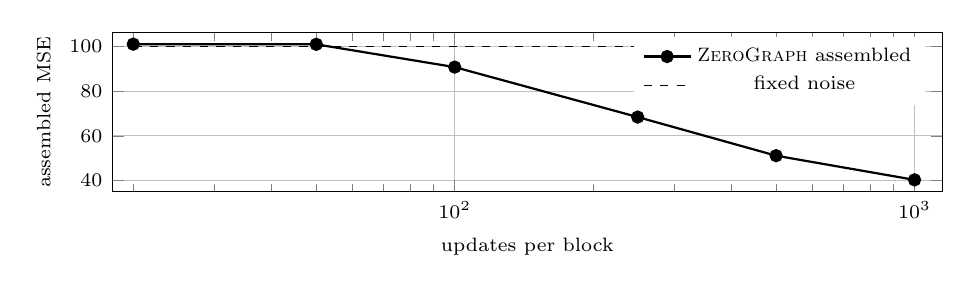
\begin{tikzpicture}
\begin{axis}[width=\columnwidth,height=3.6cm,xmode=log,log basis x=10,
xmin=18,xmax=1150,ymin=35,ymax=106,xlabel={updates per block},
ylabel={assembled MSE},tick label style={font=\scriptsize},
label style={font=\scriptsize},legend style={font=\scriptsize,draw=none,
at={(.98,.98)},anchor=north east},grid=major]
\addplot[black,thick,mark=*] coordinates {(20,100.9819) (50,100.9090)
(100,90.7282) (250,68.4172) (500,51.1592) (1000,40.3645)};
\addlegendentry{\ZG{} assembled}
\addplot[black,dashed] coordinates {(20,99.8916) (1000,99.8916)};
\addlegendentry{fixed noise}
\end{axis}
\end{tikzpicture}
\caption{Held-out trajectory for the synthetic 4.027B representation fixture.}
\label{fig:appendix-trajectory}
\end{figure}

The ten-stream schedule was 3.84\% faster than one stream and produced
identical final tensor digests. Peak allocation increased 1.952~GB. Nsight
recorded 8,150 kernels on ten streams; 27.515~ms (2.30\% of kernel-active
union) had concurrency two. No NCCL, c10d, all-reduce, all-gather, or
reduce-scatter kernel appeared. This proves concurrency but not a general
multi-GPU speed law.

\section{ExactGraph Objective-Preserving Control}

\ExactGraph{} uses the same structural partitions but preserves the ordinary
loss. It rematerializes one partition at a time and propagates exact boundary
VJPs. Certification compares initial state, output, separators, scalar loss,
gradients, optimizer state, post-step parameters, buffers and aliases, inputs,
and RNG bytes. Unsupported capture, mutation, nondeterminism, sparse gradients,
or guard drift rejects before the optimized path runs.

The fixture is a five-layer BF16 causal residual Transformer of width 4096,
32 heads, sequence length eight, and 1,006,714,880 parameters. One complete
optimizer step passed output, loss, 40 gradient tensors (2.013~GB), optimizer
state, parameters, inputs, and RNG. Ordinary forward retained 77 non-state
storages (5,510,904 bytes); rematerialized forward retained seven (589,824
bytes). Peak CUDA increments were unchanged because parameters and gradients
dominated. The one-step timing is a mechanics measurement, not stable
throughput.

An optional transport codec predicts a boundary adjoint and losslessly encodes
the XOR residual, falling back to dense bytes. Eight observed adjoints
reconstructed bitwise; the second warm step used 117,580 wire bytes versus
262,144 dense bytes. This changes the representation of an exact dependency,
not the dependency itself.

\section{Smaller Real-Data Checks}

An 11.1M-parameter conditional model trained on 4,096 MNIST examples achieved
assembled MSE 0.08575 versus 1.10389 for noise and 0.01309 for the end-to-end
source. A pretrained 81.9M-parameter DistilGPT-2 conversion trained two local
blocks for 5,000 steps. Its preregistered WikiText gate passed: teacher-scored
NLL 7.684, maximum token share 0.0983, mean unique-token fraction 0.7856, and
normalized entropy 0.3571. Teacher NLL on real validation text was 5.815,
exposing a material quality gap rather than parity.

\section{Traceability and Claim Boundaries}

The verifier checks 69 claims against retained JSON evidence and recomputes the
generated result macros. Key SHA-256 prefixes are: \ExactGraph{} certificate
\texttt{734c610c9c9}; 4B report \texttt{7bfcf4f3071}; concurrency manifest
\texttt{4051cf9a4dd}; TinyLlama orchestration \texttt{464db1743aee}; primary
evaluation \texttt{27253044ded6}; and confirmation evaluation
\texttt{c635b6afcfb3}. The six-arm verified-summary prefix is
\texttt{28be510ee595}, its independent verification is
\texttt{6c98ee71d2cf}, and primary evaluation is
\texttt{571d94b79cb9}. Complete digests, not prefixes, are verified.
The final nine-phase campaign summary has SHA-256 prefix
\texttt{702bd8265fab}; its status is \texttt{verified}, all nine phases are
complete, and its failure list is empty. The campaign generator fails closed on
those invariants and reproduces both the LaTeX macros and ordered Markdown
report from that summary.

For the GPT-2 Large pair, the checkpoint revision prefix is
\texttt{32b71b12589c}, model digest \texttt{5f47f3e12f91}, token digest
\texttt{f0d18873b700}, evaluation-code digest \texttt{8075c272042d}, and DDP
checkpoint digest \texttt{ab5c7590d83a}. Local report prefixes are
\texttt{8d0446c1}, \texttt{b72a9874}, \texttt{ae454b56}, and
\texttt{3bce6d70}. The root preregistration and 13 hash-chained operational
addenda disclose canceled engineering attempts and the budget-stopped partial
seed; only the completed matched pair contributes results.

\section{Submission Checklist}

\begin{itemize}
\item The main claim is conversion/distillation, not from-scratch pretraining.
\item Local critical-path time excludes cache construction; reported first-use
time adds the measured cache pass and excludes common evaluation/checkpoint I/O.
\item Zero inter-block bytes applies only to frozen/private-interface strict
mode.
\item The GPT-2 result is one completed negative seed; the confirmation seed
for TinyLlama is shorter than the primary.
\item The six-arm D confirmation was barred by its preregistered primary
coherence failure; C is the positive boundary-regression control.
\item The 4B experiment is synthetic systems evidence, not 4B language quality.
\item The 1B ExactGraph reduction is retained forward storage, not total HBM.
\item The new comparison includes FSDP2, boundary-shift tests, and cache
accounting; ZeRO-3, a second architecture, and broader downstream/human
evaluation remain required.
\end{itemize}

\section{Reproduction and Artifact Map}

From the repository root, the complete manuscript check is:
\begin{verbatim}
make ieee-paper
\end{verbatim}
This command regenerates the evidence verification report, compiles the main
paper and supplement with the vendored IEEE class, and rejects a main paper
over nine pages. The underlying fail-closed checks can be invoked directly:
\begin{verbatim}
cd papers/zerograph_ieee
python3 generate_l4_results.py --check
python3 generate_tinyllama_results.py \
  --check
python3 generate_six_arm_results.py \
  --check
python3 verify_evidence.py \
  --output evidence-verification.json
\end{verbatim}
The manuscript fails when any generated result file is absent; a missing
evidence input cannot silently produce a shorter paper with different claims.

\begin{table}[t]
\caption{Primary repository evidence locations.}
\label{tab:artifact-map}
\centering\scriptsize
\begin{tabular}{@{}ll@{}}
\toprule
Evidence & Repository path \\
\midrule
Claim table & \texttt{papers/zerograph\_ieee/claims.json} \\
GPT-2 protocol & \texttt{experiments/modal\_l4\_poc/} \\
GPT-2 reports & \texttt{artifacts/modal\_l4\_stopped\_seed1/} \\
TinyLlama protocol & \texttt{experiments/modal\_l4\_tinyllama/} \\
TinyLlama reports & \texttt{artifacts/modal\_l4\_tinyllama/} \\
Six-arm reports & \texttt{artifacts/modal\_l4\_six\_arm/} \\
4B report & \texttt{artifacts/independent\_4b\_training/} \\
ExactGraph control & \texttt{artifacts/exact\_1b\_cuda\_v0\_17\_0\_final/} \\
\bottomrule
\end{tabular}
\end{table}

\section{Evidence-First Strengthening Campaign}

The nine-phase protocol used revision-pinned Qwen2.5-1.5B checkpoints,
UltraChat, length 256, 2,048 updates, and four L4s. It compared FSDP2/ZeRO-3
SFT, connected distillation, online boundaries, and cached \ZG{}. It covered
three seeds, $B\in\{2,4,8\}$, five interpolation weights, noise stress, five
downstream tasks, 16 reuse pairs, INT8 compression, and failure/restart.

The objective-matched cached/online jobs held teacher, examples, targets,
optimizer, updates, evaluation, and allocation fixed. Twelve cache boundaries
matched bitwise. Deterministic kernels were reserved for restart certification.

At 3B, fixed base/teacher revisions were partitioned
$[0,9),[9,18),[18,27),[27,36)$; each 693.7M-parameter job consumed 524,288
tokens. All local losses fell and assembly passed CE, context, and coherence
gates. The claim remains pretrained conversion/distillation.

The lifecycle test sent SIGTERM to block~1 at step 256, restored it to step
512, and compared it with an uninterrupted control. Canonical final tensor
digests matched bitwise; unaffected jobs were not rerun. Two failed engineering
attempts---GPU-mapped RNG state and initially nondeterministic kernels---remain
in the append-only ledger rather than being erased.

\section{Six-Arm FSDP2 Comparison Protocol}
\label{app:six-arm}

The A--F comparison uses the same revision-pinned TinyLlama base, Chat teacher,
UltraChat split, 256-token shape, and deterministic four-example stream as the
conversion study. Each primary arm receives 2,048 updates (2,097,152 example
tokens). Owned parameters and AdamW state are FP32; forward/backward compute is
BF16, and FSDP2 reductions are FP32. Optimizer settings are AdamW with learning
rate $2\times10^{-5}$, $\beta=(0.9,0.95)$, zero weight decay, and gradient-norm
cap 1.0.

Arm A is global assistant-only cross entropy with activation checkpointing and
four-way FSDP2. Arm B assigns the unanchored local denoising objective to four
independent jobs. Arm C uses the cached teacher trajectory at $\sigma=0$,
providing a hidden-state-regression control. Arm D uses the same cache with
log-uniform $\sigma\in[0.005,0.10]$. Arm E recomputes the identical D targets
online. Arm F changes D to two depth partitions, each sharded over a disjoint
two-GPU FSDP2 group. Thus C versus D isolates noise conditioning, D versus E
isolates materialization, and D versus F tests composition with state sharding.

The first 128-step pilot exposed a declared-gate mismatch: the final block's
mixed scalar loss includes batch-variable assistant CE, despite the gate's
intended use as a denoising-learning check. The original failure is retained.
Before further allocation, an append-only addendum locked a 256-step diagnostic
and required every block's denoising component to decrease while all previously
locked held-out, context, and coherence gates remained unchanged. Arm B failed
local/coherence gates and could not escalate. This amendment is post-pilot and
must not be described as part of the original preregistration.

Boundary robustness mixes teacher and assembled predecessor states at fractions
$\alpha\in\{1,0.75,0.5,0.25,0\}$ and reports teacher-target MSE for every
block. Communication accounting separates strict inter-block gradient bytes
from algorithmic intra-block FSDP2 tensor payload. Materialization economics
reports the cache pass, local critical path, first use, and amortized reuse at
$K\in\{1,2,4,8\}$. The incremental Modal ledger has a hard \$25 ceiling.

All A/C/D/E/F primaries completed without OOM, and the final ledger was
\SixSpend{}. C passed every assembled gate. D and E were bitwise identical but
failed coherence; F also failed coherence. The preregistered rule conditioned a
second D seed on the primary quality gate, so it was not launched. This is a
stopped negative result, not missing-at-random replication. The compact bundle
retains both preregistrations, every gate report, per-arm telemetry summaries,
the cost ledger, exact executed-source hashes, and an independent verification
record.

% Generated by IEEEtran.bst, version: 1.14 (2015/08/26)
\begin{thebibliography}{10}
\providecommand{\url}[1]{#1}
\csname url@samestyle\endcsname
\providecommand{\newblock}{\relax}
\providecommand{\bibinfo}[2]{#2}
\providecommand{\BIBentrySTDinterwordspacing}{\spaceskip=0pt\relax}
\providecommand{\BIBentryALTinterwordstretchfactor}{4}
\providecommand{\BIBentryALTinterwordspacing}{\spaceskip=\fontdimen2\font plus
\BIBentryALTinterwordstretchfactor\fontdimen3\font minus
  \fontdimen4\font\relax}
\providecommand{\BIBforeignlanguage}[2]{{%
\expandafter\ifx\csname l@#1\endcsname\relax
\typeout{** WARNING: IEEEtran.bst: No hyphenation pattern has been}%
\typeout{** loaded for the language `#1'. Using the pattern for}%
\typeout{** the default language instead.}%
\else
\language=\csname l@#1\endcsname
\fi
#2}}
\providecommand{\BIBdecl}{\relax}
\BIBdecl

\bibitem{chen2016}
T.~Chen, B.~Xu, C.~Zhang, and C.~Guestrin, ``Training deep nets with sublinear
  memory cost,'' in \emph{Proc. NIPS Workshop on Memory-Efficient Machine
  Learning}, 2016.

\bibitem{zero}
S.~Rajbhandari, J.~Rasley, O.~Ruwase, and Y.~He, ``{ZeRO}: Memory optimizations
  toward training trillion parameter models,'' in \emph{Proc. SC}, 2020, pp.
  1--16.

\bibitem{fsdp}
Y.~Zhao, A.~Gu, R.~Varma, L.~Luo, C.-C. Huang, M.~Xu, L.~Wright,
  H.~Shojanazeri, M.~Ott, S.~Shleifer, A.~Desmaison, C.~Balioglu, B.~Nguyen,
  G.~Chauhan, Y.~Hao, and S.~Li, ``{PyTorch FSDP}: Experiences on scaling fully
  sharded data parallel,'' \emph{Proc. VLDB Endowment}, vol.~16, no.~12, pp.
  3848--3860, 2023.

\bibitem{megatron}
M.~Shoeybi, M.~Patwary, R.~Puri, P.~LeGresley, J.~Casper, and B.~Catanzaro,
  ``Megatron-lm: Training multi-billion parameter language models using model
  parallelism,'' \emph{arXiv preprint arXiv:1909.08053}, 2019.

\bibitem{gpipe}
Y.~Huang, Y.~Cheng, A.~Bapna, O.~Firat, M.~X. Chen, D.~Chen, H.~Lee, J.~Ngiam,
  Q.~V. Le, Y.~Wu, and Z.~Chen, ``{GPipe}: Efficient training of giant neural
  networks using pipeline parallelism,'' in \emph{Advances in Neural
  Information Processing Systems}, vol.~32, 2019.

\bibitem{diffusionblocks}
M.~Shing, M.~Koyama, and T.~Akiba, ``Diffusionblocks: Block-wise neural network
  training via diffusion interpretation,'' \emph{Proc. ICLR}, 2026,
  arXiv:2506.14202.

\bibitem{song}
Y.~Song, J.~Sohl-Dickstein, D.~P. Kingma, A.~Kumar, S.~Ermon, and B.~Poole,
  ``Score-based generative modeling through stochastic differential
  equations,'' in \emph{Proc. ICLR}, 2021.

\bibitem{karras}
T.~Karras, M.~Aittala, T.~Aila, and S.~Laine, ``Elucidating the design space of
  diffusion-based generative models,'' in \emph{Advances in Neural Information
  Processing Systems}, vol.~35, 2022, pp. 26\,565--26\,577.

\bibitem{pytorch}
A.~Paszke, S.~Gross, F.~Massa, A.~Lerer, J.~Bradbury, G.~Chanan, T.~Killeen,
  Z.~Lin, N.~Gimelshein, L.~Antiga \emph{et~al.}, ``{PyTorch}: An imperative
  style, high-performance deep learning library,'' in \emph{Advances in Neural
  Information Processing Systems}, vol.~32, 2019.

\bibitem{dtr}
M.~Kirisame, S.~Lyubomirsky, A.~Haan, J.~Brennan, M.~He, J.~Roesch, T.~Chen,
  and Z.~Tatlock, ``Dynamic tensor rematerialization,'' in \emph{Proc. ICLR},
  2021.

\bibitem{dni}
M.~Jaderberg, W.~M. Czarnecki, S.~Osindero, O.~Vinyals, A.~Graves, D.~Silver,
  and K.~Kavukcuoglu, ``Decoupled neural interfaces using synthetic
  gradients,'' in \emph{Proc. ICML}, 2017, pp. 1627--1635.

\bibitem{greedy}
E.~Belilovsky, M.~Eickenberg, and E.~Oyallon, ``Greedy layerwise learning can
  scale to imagenet,'' in \emph{Proc. AISTATS}, 2019, pp. 583--593.

\bibitem{blocktrain}
P.~Toth and D.~Oprisa, ``Decentralised ai training and inference with
  blocktrain,'' \emph{arXiv preprint arXiv:2606.24722}, 2026.

\bibitem{hinton2015}
G.~Hinton, O.~Vinyals, and J.~Dean, ``Distilling the knowledge in a neural
  network,'' \emph{arXiv preprint arXiv:1503.02531}, 2015.

\bibitem{fitnets}
A.~Romero, N.~Ballas, S.~E. Kahou, A.~Chassang, C.~Gatta, and Y.~Bengio,
  ``{FitNets}: Hints for thin deep nets,'' in \emph{Proc. ICLR}, 2015.

\bibitem{patientkd}
S.~Sun, Y.~Cheng, Z.~Gan, and J.~Liu, ``Patient knowledge distillation for
  {BERT} model compression,'' in \emph{Proc. EMNLP-IJCNLP}, 2019, pp.
  4323--4332.

\bibitem{tinybert}
X.~Jiao, Y.~Yin, L.~Shang, X.~Jiang, X.~Chen, L.~Li, F.~Wang, and Q.~Liu,
  ``{TinyBERT}: Distilling {BERT} for natural language understanding,'' in
  \emph{Findings of EMNLP}, 2020, pp. 4163--4174.

\end{thebibliography}

\end{document}
